\chapter{Mengenal Kecerdasan Buatan dan Scikit-Learn}
Buku umum yang digunakan adalah \cite{russell2016artificial} dan  
untuk sebelum UTS menggunakan buku \textit{Python Artificial Intelligence Projects for Beginners}\cite{eckroth2018python}.
Dengan praktek menggunakan python 3 dan editor anaconda dan library python scikit-learn.
Tujuan pembelajaran pada pertemuan pertama antara lain:
\begin{enumerate}
\item
Mengerti definisi kecerdasan buatan, sejarah kecerdasan buatan, perkembangan dan penggunaan di perusahaan
\item
Memahami cara instalasi dan pemakaian sci-kit learn
\item
Memahami cara penggunaan variabel explorer di spyder
\end{enumerate}
Tugas dengan cara dikumpulkan dengan pull request ke github dengan menggunakan latex pada repo yang dibuat oleh asisten riset.

\section{Teori}
Praktek teori penunjang yang dikerjakan :
\begin{enumerate}
\item
Buat Resume Definisi, Sejarah dan perkembangan Kecerdasan Buatan, dengan bahasa yang mudah dipahami dan dimengerti. Buatan sendiri bebas plagiat[hari ke 1](10)
\item
Buat Resume mengenai definisi supervised learning, klasifikasi, regresi dan unsupervised learning. Data set, training set dan testing set.[hari ke 1](10)
\end{enumerate}

\section{Instalasi}
Membuka https://scikit-learn.org/stable/tutorial/basic/tutorial.html. Dengan menggunakan bahasa yang mudah dimengerti dan bebas plagiat. 
Dan wajib skrinsut dari komputer sendiri.
\begin{enumerate}
\item
Instalasi library scikit dari anaconda, mencoba kompilasi dan uji coba ambil contoh kode dan lihat variabel explorer[hari ke 1](10)
\item
Mencoba Loading an example dataset, menjelaskan maksud dari tulisan tersebut dan mengartikan per baris[hari ke 1](10)
\item
Mencoba Learning and predicting, menjelaskan maksud dari tulisan tersebut dan mengartikan per baris[hari ke 2](10)
\item
mencoba Model persistence, menjelaskan maksud dari tulisan tersebut dan mengartikan per baris[hari ke 2](10)
\item 
Mencoba Conventions, menjelaskan maksud dari tulisan tersebut dan mengartikan per baris[hari ke 2](10)
\end{enumerate}


\section{Penanganan Error}
Dari percobaan yang dilakukan di atas, apabila mendapatkan error maka:

\begin{enumerate}
	\item
	skrinsut error[hari ke 2](10)
	\item
Tuliskan kode eror dan jenis errornya [hari ke 2](10)
	\item
Solusi pemecahan masalah error tersebut[hari ke 2](10)

\end{enumerate}

\section{Ahmad Syafrizal Huda/1164062}
\subsection{Teori}
\begin{enumerate}
\item Definisi, sejarah, dan perkembangan kecerdasan buatan.
\subitem Definisi kecerdasan buatan adalah suatu pengetahuan yang dapat membuat komputer untuk meniru kecerdasan manusia yang berhubungan dengan penangkapan, pemodelan, dan penyimpanan kecerdasan manusia dalam sebuah sistem teknologi. Contohnya yaitu melakukan analisa penalaran untuk mengambil suatu kesimpulan atau penerjemahan atau keputusan dari satu bahasa satu ke bahasa lain.
\subitem Sejarah dan perkembangan kecerdasan buatan terjadi pada musim panas tahun 1956 tercatat adanya seminar mengenai AI di Darmouth College. Seminar pada waktu itu dihadiri oleh sejumlah pakar komputer dan membahas potensi komputer dalam meniru kepandaian manusia. Akan tetapi perkembangan yang sering terjadi semenjak diciptakannya LISP, yaitu bahasa kecerdasan buatan yang dibuat tahun 1960 oleh John McCarthy. Istilah pada kecerdasan buatan atau Artificial Intelligence diambil dari Marvin Minsky dari MIT. Dia menulis karya ilmiah berjudul Step towards Artificial Intelligence, The Institute of radio Engineers Proceedings 49, January 1961\cite{baraja2008kecerdasan}. 
\item  Definisi supervised learning, klasifikasi, regresi, dan unsupervised learning. Data set, training set dan testing set. 
\subitem Supervised learning merupakan sebuah pendekatan dimana sudah terdapat data yang dilatih, dan terdapat variable yang ditargetkan sehingga tujuan dari pendekatan ini adalah mengkelompokan suatu data ke data yang sudah ada. Sedangkan unsupervised learning tidak memiliki data latih, sehingga dari data yang ada, kita mengelompokan data tersebut menjadi 2 bagian atau 3 bagian dan seterusnya.
\subitem Klasifikasi adalah salah satu topik utama dalam data mining atau machine learning. Klasifikasi yaitu suatu pengelompokan data dimana data yang digunakan tersebut mempunyai kelas label atau target.
\subitem Regresi adalah Supervised learning tidak hanya mempelajari classifier, tetapi juga mempelajari fungsi yang dapat memprediksi suatu nilai numerik. Contoh, ketika diberi foto seseorang, kita ingin memprediksi umur, tinggi, dan berat orang yang ada pada foto tersebut.
\subitem Data set adalah cabang aplikasi dari Artificial Intelligence/Kecerdasan Buatan yang fokus pada pengembangan sebuah sistem yang mampu belajar sendiri tanpa harus berulang kali di program oleh manusia.
\subitem Training set yaitu jika pasangan objek, dan kelas yang menunjuk pada objek tersebut adalah suatu contoh yang telah diberi label akan menghasilkan suatu algoritma pembelajaran.
\subitem Testing set digunakan untuk mengukur sejauh mana classifier berhasil melakukan klasifikasi dengan benar\cite{zhu2009introduction}.
\end{enumerate}
\subsection{Instalasi}
\subsubsection{Instalasi Library Scikit dari Anaconda}
\begin{enumerate}
\item Download aplikasi Anaconda terlebih dahulu. Lihat pada gambar 1.4.
\item Install aplikasi Anaconda yang sudah di download tadi. Lihat pada gambar 1.5.
\item Simpan aplikasi sesuai folder yang kita pilih lalu next. Lihat pada gambar 1.6.
\item Centang Keduanya lalu tekan tombol install. Lihat pada gambar 1.7.
\item Setelah itu tunggu sampai proses instalasi selesai lalu jika sudah tekan tombol finish. Lihat pada gambar 1.8.
\item Lalu buka command prompt anda dan tuliskan perintah berikut ini untuk mengecek apakah aplikasinya sudah terinstall. Lihat pada gambar 1.9.
\item Kemudian ketikkan perinta pip install -U scikit-learn seperti gambar berikut. Lihat pada gambar 1.10.
\item Lalujika sudah  ketikkan juga perintah conda install scikit-learn. Lihat pada gambar 1.11.
\item Hasil compile dari beberapa code yang mempunyai variable explorer. Lihat pada gambar 1.12.
\end{enumerate}
\subsubsection{Mencoba Loading an example Dataset}
\begin{itemize}
\item\begin{verbatim}from sklearn import datasets\end{verbatim}(pada baris ini merupakan sebuah perintah untuk mengimport class datasets dari packaged sklearn).
\item\begin{verbatim} iris = datasets.load_iris()\end{verbatim}(pada baris kedua ini dimana iris merupakan suatu estimator/parameter yang berfungsi untuk mengambil data pada item datasets.load\_iris).
\item\begin{verbatim} digits = datasets.load_digits()\end{verbatim}(pada baris ketiga ini dimana digits merupakan suatu estimator/parameter yang berfungsi untuk mengambil data pada item datasets.load\_digits).
\item\begin{verbatim} print(digits.data)\end{verbatim}(pada baris keempat ini merupakan perintah yang berfungsi untuk menampilkan estimator/parameter yang dipanggil pada item digits.data dan menampilkan outputannya) Lihat gambar 1.13.
\item\begin{verbatim} digits.target\end{verbatim}(barisan ini untuk mengambil target pada estimator/parameter digits dan menampilkan outputannya) Lihat gambar 1.14.
\item\begin{verbatim} digits.images[0]\end{verbatim}(barisan ini untuk mengambil images[0] pada estimator/parameter digits dan menampilkan outputannyal) Lihat gambar 1.15.
\end{itemize}
\subsubsection{Learning and Predicting}
\begin{itemize}
\item\begin{verbatim} from sklearn import svm\end{verbatim}(pada baris ini merupakan sebuah perintah untuk mengimport class svm dari packaged sklearn).
\item\begin{verbatim} clf = svm.SVC(gamma=0.001, C=100.)\end{verbatim}(pada baris kedua ini clf sebagai estimator/parameter, svm.SVC sebagai class, gamma sebagai parameter untuk menetapkan nilai secara manual).
\item\begin{verbatim} clf.fit(digits.data[:-1], digits.target[:-1])\end{verbatim}(pada baris ketiga ini clf sebagai estimator/parameter, fit sebagai metode, digits.data sebagai item, [:-1] sebagai syntax pythonnya dan menampilkan outputannya) Lihat gambar 1.16.
\item\begin{verbatim} clf.predict(digits.data[-1:])\end{verbatim}(pada baris terakhir ini clf sebagai estimator/parameter, predict sebagai metode lainnya, digits.data sebagai item dan menampilkan outputannya) Lihat gambar 1.17.
\end{itemize}
\subsubsection{Model Presistence}
\begin{itemize}
\item\begin{verbatim} from sklearn import svm\end{verbatim}(pada baris ini merupakan sebuah perintah untuk mengimport class svm dari packaged sklearn).
\item\begin{verbatim} from sklearn import datasets\end{verbatim}(pada baris ini merupakan sebuah perintah untuk mengimport class datasets dari packaged sklearn).
\item\begin{verbatim} clf = svm.SVC(gamma='scale')\end{verbatim}(pada baris ketga ini clf sebagai estimator/parameter, svm.SVC sebagai class, gamma sebagai parameter untuk menetapkan nilai secara manual dengan nilai scale).
\item\begin{verbatim} iris = datasets.load_iris()\end{verbatim}(pada baris keempat ini iris sebagai estimator/parameter, datasets.load\_iris() sebagai item dari suatu nilai).
\item\begin{verbatim} X, y = iris.data, iris.target\end{verbatim}(pada baris kelima ini X, y sebagai estimator/parameter, iris.data, iris.target sebagai item dari 2 nilai yang ada).
\item\begin{verbatim} clf.fit(X, y)\end{verbatim}(pada baris keenam ini clf sebagai estimator/parameter dengan menggunakan metode fit untuk memanggil estimator X, y dengan outputannya) Lihat gambar 1.18.
\item\begin{verbatim} import pickle\end{verbatim}(pickle merupakaan sebuah class yang di import).
\item\begin{verbatim} s = pickle.dumps(clf)\end{verbatim}(pada baris ini s sebagai estimator/parameter dengan pickle.dumps merupakan suatu nilai/item dari estimator/parameter clf)
\item\begin{verbatim} clf2 = pickle.loads(s)\end{verbatim}(pada baris ini clf2 sebagai estimator/parameter, pickle.loads sebagai suatu item, dan s sebagai estimator/parameter yang dipanggil) 
\item\begin{verbatim} clf2.predict(X[0:1])\end{verbatim}(pada baris ini clf2.predict sebagai suatu item dengan menggunakan metode predict untuk menentukkan suatu nilai dari (X[0:1])) Lihat gambar 1.19.
\item\begin{verbatim} y[0]\end{verbatim}(pada estimator/parameter y berapapun angka yang diganti nilainya akan selalu konstan yaitu 0) Lihat gambar 1.20. 
\item\begin{verbatim} from joblib import dump, load\end{verbatim}(pada baris berikut ini merupakan sebuah perintah untuk mengimport class dump, load dari packaged joblib).
\item\begin{verbatim} dump(clf, 'filename.joblib')\end{verbatim}(pada baris berikutnya dump di sini sebagai class yang didalamnya terdapat nilai dari suatu item clf dan data joblib).
\item\begin{verbatim} clf = load('filename.joblib')\end{verbatim}(pada baris terakhir clf sebagai estimato/parameter dengan suatu nilai load berfungsi untuk mengulang data sebelumnya)
\item dari ketiga baris akhir tersebut jika di jalankan aau dituliskan perintah seperti itu maka akan menampilkan tampilan eror terlihat pada gambar 1.21.
\end{itemize}
\subsubsection{Conventions}
\begin{enumerate}
\item Type Casting
\begin{itemize}
\item\begin{verbatim} from sklearn import svm\end{verbatim}(pada baris ini merupakan sebuah perintah untuk mengimport class svm dari packaged sklearn).
\item\begin{verbatim} from sklearn import random_projection\end{verbatim}(pada baris ini merupakan sebuah perintah untuk mengimport class random\_projection dari packaged sklearn).
\item\begin{verbatim} rng = np.random.RandomState(0)\end{verbatim}(rng sebagai estimator/parameter dengan nilai suatu itemnya yaitu np.random.RandomState(0)).
\item\begin{verbatim} X = rng.rand(10, 2000)\end{verbatim}(X sebagai estimator/parameter dengan nilai item rng.rand).
\item\begin{verbatim} X = np.array(X, dtype='float32')\end{verbatim}(X sebagai estimator/parameter dengan nilai item np.array).
\item\begin{verbatim} X.dtype\end{verbatim}(X.dtype sebagai item pemanggil) Lihat gambar 1.22.
\item\begin{verbatim} transformer = random_projection.GaussianRandomProjection()\end{verbatim}(transformer sebagai estimator/parameter dengan memanggil class random\_projection).
\item\begin{verbatim} X_new = transformer.fit_transform(X)\end{verbatim}(X\_new di sini sebagai estomator/parameter dan menggunakan metode fit)
\item\begin{verbatim} X_new.dtype\end{verbatim}(X\_new.dtype sebagai item) Lihat gambar1.23.
\item\begin{verbatim} from sklearn import datasets\end{verbatim}(pada baris ini merupakan sebuah perintah untuk mengimport class datasets dari packaged sklearn).
\item\begin{verbatim} from sklearn.svm import SVC\end{verbatim}(pada baris ini merupakan sebuah perintah untuk mengimport class SVC dari packaged sklearn.svm).
\item\begin{verbatim} iris = datasets.load_iris()\end{verbatim}(iris sebagai estimator/parameter dengan item datasets.load\_iris()).
\item\begin{verbatim} clf = SVC(gamma='scale')\end{verbatim}(clf sebagai estimator/parameter dengan nilai class SVC pada parameter gamma sebagai set penilaian).
\item\begin{verbatim} clf.fit(iris.data, iris.target)\end{verbatim}(estimator/parameter clf menggunakan metode fit dengan itemnya) Lihat gambar 1.24.
\item\begin{verbatim} list(clf.predict(iris.data[:3]))\end{verbatim}(menambahkan item list dengan metode predict) Lihat gambar 1.25.
\item\begin{verbatim} clf.fit(iris.data, iris.target_names[iris.target])\end{verbatim}(estimator/parameter clf menggunakan metode fit dengan itemnya) Lihat gambar 1.26.
\item\begin{verbatim} list(clf.predict(iris.data[:3]))(menambahkan item list dengan metode predict\end{verbatim} Lihat gambar 1.27.
\end{itemize}
\item Refitting and Updating Parameters
\begin{itemize}
\item\begin{verbatim} import numpy as np\end{verbatim}(pada baris ini merupakan sebuah perintah untuk mengimport class svm dari np).
\item\begin{verbatim} from sklearn.svm import SVC\end{verbatim}(pada baris ini merupakan sebuah perintah untuk mengimport class SVC dari packaged sklearn.svm).
\item\begin{verbatim} rng = np.random.RandomState(0)\end{verbatim}(rng sebagai estimator/parameter dengan nilai suatu itemnya yaitu np.random.RandomState(0)).
\item\begin{verbatim} X = rng.rand(100, 10)\end{verbatim}(X sebagai estimator/parameter dengan nilai item rng.rand).
\item\begin{verbatim} y = rng.binomial(1, 0.5, 100)\end{verbatim}(y sebagai estimator/parameter dengan nilai item rng.binomial).
\item\begin{verbatim} X_test = rng.rand(5, 10)\end{verbatim}(X\_test sebagai estimator/parameter dengan nilai item rng.rand).
\item\begin{verbatim} clf = SVC()\end{verbatim}(clf sebagai estimator/parameter dan class SVC)
\item\begin{verbatim} clf.set_params(kernel='linear').fit(X, y)\end{verbatim}(set\_params sebagai item) Lihat gambar 1.28.
\item\begin{verbatim} clf.predict(X_test)\end{verbatim}(menggunakan metode predict) Lihat gambar 1.29.
\item\begin{verbatim} clf.set_params(kernel='rbf', gamma='scale').fit(X, y)\end{verbatim} Lihat gambar 1.30.
\item\begin{verbatim} clf.predict(X_test)\end{verbatim} Lihat gambar 1.31.
\end{itemize}
\item Multiclass vs. Multilabel Fitting
\begin{itemize}
\item\begin{verbatim} from sklearn.svm import SVC\end{verbatim}(pada baris ini merupakan sebuah perintah untuk mengimport class SVC dari packaged sklearn.svm).
\item\begin{verbatim} from sklearn.multiclass import OneVsRestClassifier\end{verbatim}(pada baris ini merupakan sebuah perintah untuk mengimport class OneVsRestClassifier dari packaged sklearn.multiclass).
\item\begin{verbatim} from sklearn.preprocessing import LabelBinarizer\end{verbatim}(pada baris ini merupakan sebuah perintah untuk mengimport class LabelBinarizer dari packaged sklearn.preprocessing).
\item\begin{verbatim} X = [[1, 2], [2, 4], [4, 5], [3, 2], [3, 1]]\end{verbatim}
\item\begin{verbatim} y = [0, 0, 1, 1, 2]\end{verbatim}
\item\begin{verbatim} classif = OneVsRestClassifier(estimator=SVC(gamma='scale',random_state=0))\end{verbatim}
\item\begin{verbatim} classif.fit(X, y).predict(X)\end{verbatim} Lihat gambar 1.32.
\item\begin{verbatim} y = LabelBinarizer().fit_transform(y)\end{verbatim}
\item\begin{verbatim} classif.fit(X, y).predict(X)\end{verbatim} Lihat gambar 1.33.
\item\begin{verbatim} from sklearn.preprocessing import MultiLabelBinarizer\end{verbatim}
\item\begin{verbatim} y = [[0, 1], [0, 2], [1, 3], [0, 2, 3], [2, 4]]\end{verbatim}
\item\begin{verbatim} y = MultiLabelBinarizer().fit_transform(y)\end{verbatim}
\item\begin{verbatim} classif.fit(X, y).predict(X)\end{verbatim} Lihat gambar 1.34.
\end{itemize}
\end{enumerate}

\subsection{Penanganan eror}
\subsubsection{ScreenShoot Eror}
\begin{figure}[ht]\centerline{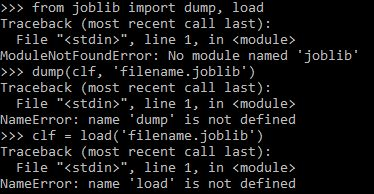
\includegraphics[width=0.75\textwidth]{figures/huda/18.JPG}}\caption{Hasil Tampilan Error.}\end{figure}
\subsubsection{Tuliskan Kode Eror dan Jenis Erornya}
\begin{itemize}
\item \begin{verbatim}from joblib import dump, load\end{verbatim} (Kode baris pertama)
\subitem \begin{verbatim}
Traceback(most recent call last):
 File "<stdin>", line 1, in<module>
ModuleNotFoundError: No module named 'joblib'
\end{verbatim} (Errornya)
\item \begin{verbatim}dump(clf, 'filename.joblib')\end{verbatim} (Kode baris kedua)
\subitem \begin{verbatim}
Traceback(most recent call last):
 File "<stdin>", line 1, in<module>
NameError: name 'dump' is not defined
\end{verbatim} (Errornya)
\item \begin{verbatim}clf = load('filename.joblib')\end{verbatim} (Kode baris ketiga)
\subitem \begin{verbatim}
Traceback(most recent call last):
 File "<stdin>", line 1, in<module>
NameError: name 'load' is not defined
\end{verbatim} (Errornya)
\end{itemize}
\subsubsection{Solusi Pemecahan Masalah Error}
\begin{enumerate}
\item Pada masalah error sebelumnya itu dikarenakan kita belum mempunyai packaged joblib. Jadi solusinya yaitu dengan cara menginstall terlebih dahulu packaged joblibnya setelah itu baru perintah tersebut dapat dijalankan seperti pada gambar 1.2 dan 1.3
\begin{figure}[ht]\centerline{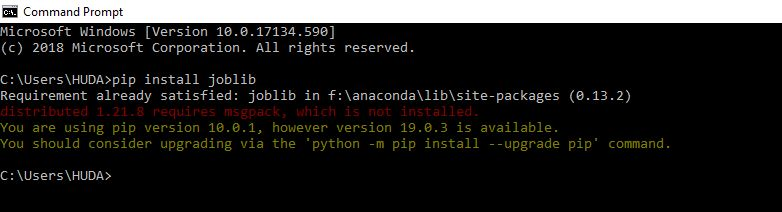
\includegraphics[width=0.75\textwidth]{figures/huda/33.JPG}}\caption{Hasil Tampilan Install joblib.}\end{figure}
\begin{figure}[ht]\centerline{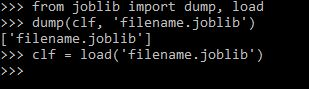
\includegraphics[width=0.75\textwidth]{figures/huda/32.JPG}}\caption{Hasil Tampilan Uji coba perintah joblib.}\end{figure}
\end{enumerate}

\begin{figure}[ht]\centerline{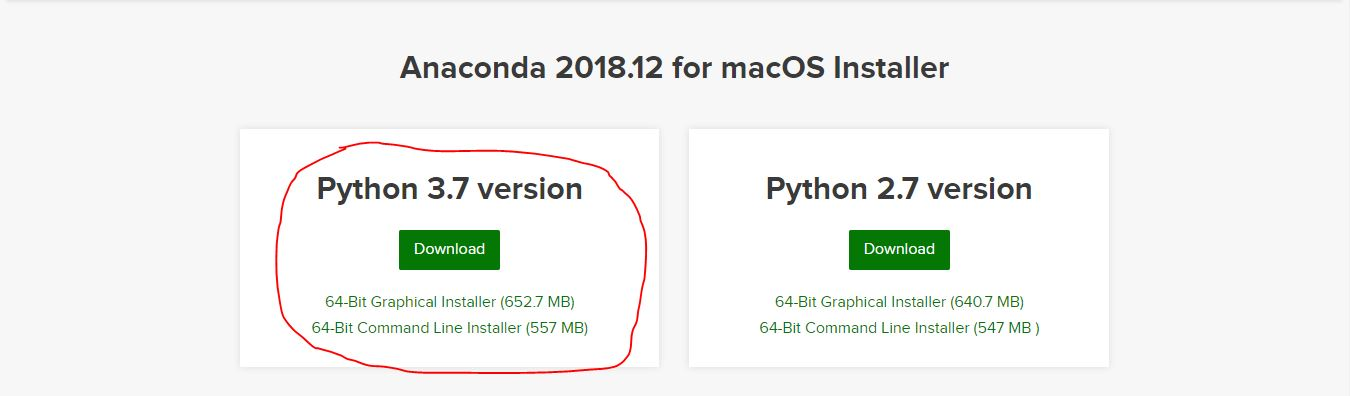
\includegraphics[width=1\textwidth]{figures/huda/1.JPG}}\caption{Download Anaconda.}\end{figure}
\begin{figure}[ht]\centerline{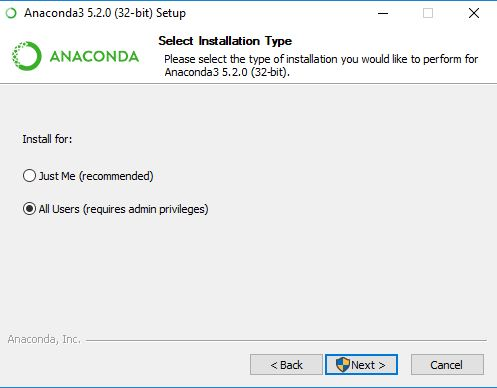
\includegraphics[width=0.75\textwidth]{figures/huda/2.JPG}}\caption{Langkah pertama instalasi anaconda.}\end{figure}
\begin{figure}[ht]\centerline{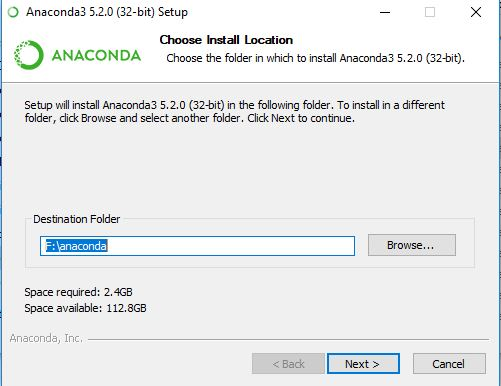
\includegraphics[width=0.75\textwidth]{figures/huda/3.JPG}}\caption{Langkah kedua instalasi anaconda.}\end{figure}
\begin{figure}[ht]\centerline{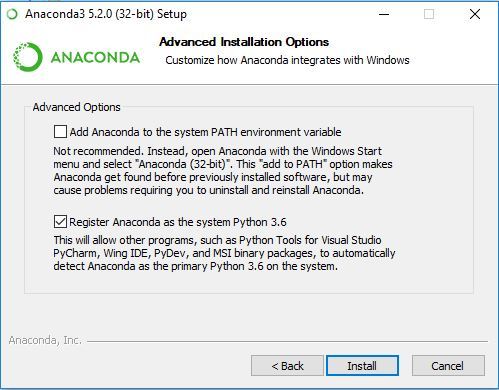
\includegraphics[width=0.75\textwidth]{figures/huda/4.JPG}}\caption{Langkah ketiga instalasi anaconda.}\end{figure}
\begin{figure}[ht]\centerline{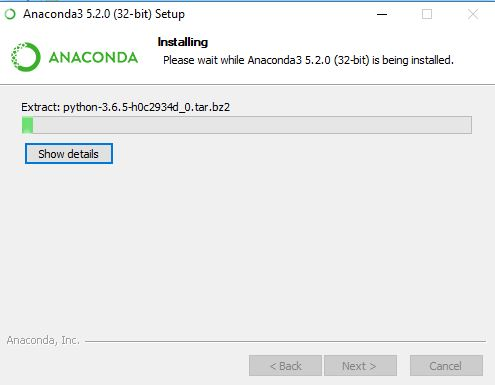
\includegraphics[width=0.75\textwidth]{figures/huda/5.JPG}}\caption{Langkah terakhir instalasi anaconda.}\end{figure}
\begin{figure}[ht]\centerline{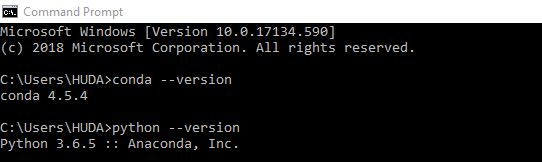
\includegraphics[width=0.75\textwidth]{figures/huda/6.JPG}}\caption{Langkah pertama instalasi scikit pada CMD.}\end{figure}
\begin{figure}[ht]\centerline{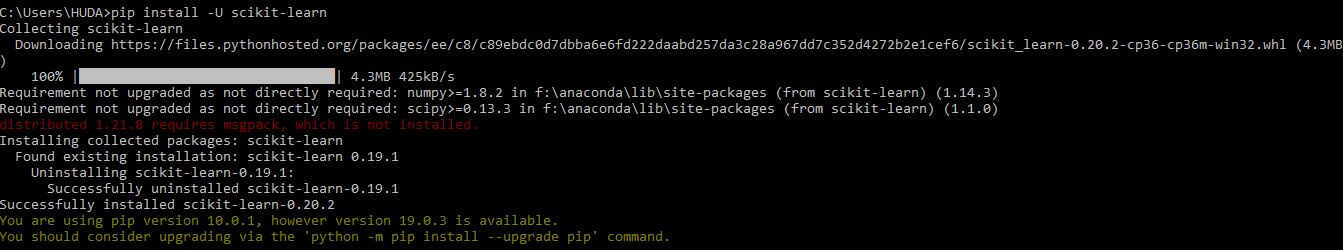
\includegraphics[width=0.75\textwidth]{figures/huda/7.JPG}}\caption{Langkah kedua instalasi scikit pada CMD.}\end{figure}
\begin{figure}[ht]\centerline{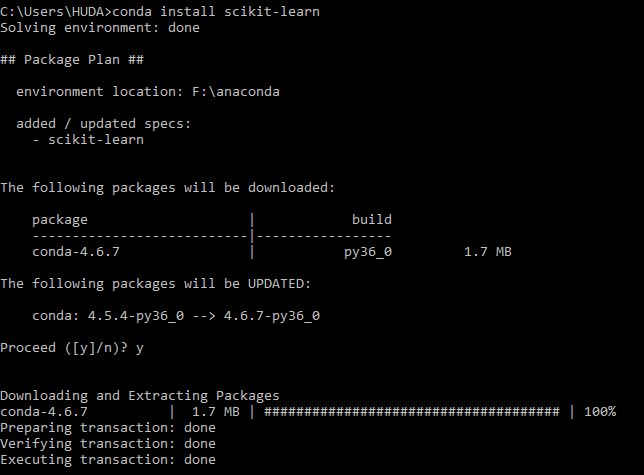
\includegraphics[width=0.75\textwidth]{figures/huda/8.JPG}}\caption{Langkah ketiga instalasi scikit pada CMD.}\end{figure}
\begin{figure}[ht]\centerline{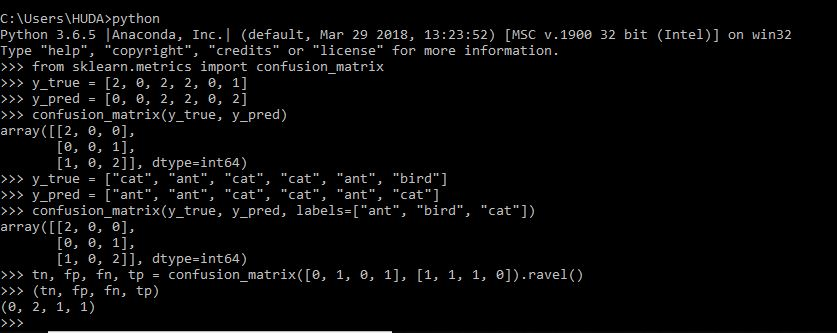
\includegraphics[width=0.75\textwidth]{figures/huda/9.JPG}}\caption{Langkah compile code pada python anaconda.}\end{figure}
\begin{figure}[ht]\centerline{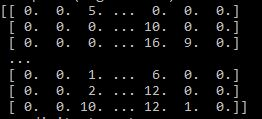
\includegraphics[width=0.75\textwidth]{figures/huda/10.JPG}}\caption{Hasil Tampilan 1.}\end{figure}
\begin{figure}[ht]\centerline{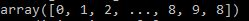
\includegraphics[width=0.75\textwidth]{figures/huda/11.JPG}}\caption{Hasil Tampilan 2.}\end{figure}
\begin{figure}[ht]\centerline{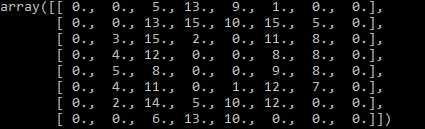
\includegraphics[width=0.75\textwidth]{figures/huda/12.JPG}}\caption{Hasil Tampilan 3.}\end{figure}
\begin{figure}[ht]\centerline{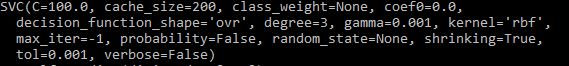
\includegraphics[width=0.75\textwidth]{figures/huda/13.JPG}}\caption{Hasil Tampilan 4.}\end{figure}
\begin{figure}[ht]\centerline{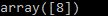
\includegraphics[width=0.75\textwidth]{figures/huda/14.JPG}}\caption{Hasil Tampilan 5.}\end{figure}
\begin{figure}[ht]\centerline{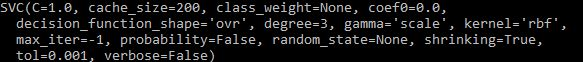
\includegraphics[width=0.75\textwidth]{figures/huda/15.JPG}}\caption{Hasil Tampilan 6.}\end{figure}
\begin{figure}[ht]\centerline{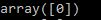
\includegraphics[width=0.75\textwidth]{figures/huda/16.JPG}}\caption{Hasil Tampilan 7.}\end{figure}
\begin{figure}[ht]\centerline{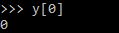
\includegraphics[width=0.75\textwidth]{figures/huda/17.JPG}}\caption{Hasil Tampilan 8.}\end{figure}
\begin{figure}[ht]\centerline{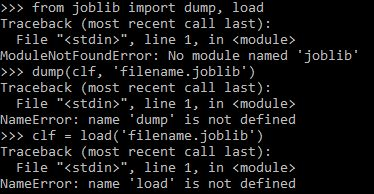
\includegraphics[width=0.75\textwidth]{figures/huda/18.JPG}}\caption{Hasil Tampilan 9.}\end{figure}
\begin{figure}[ht]\centerline{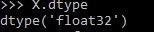
\includegraphics[width=0.75\textwidth]{figures/huda/19.JPG}}\caption{Hasil Tampilan 10.}\end{figure}
\begin{figure}[ht]\centerline{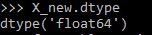
\includegraphics[width=0.75\textwidth]{figures/huda/20.JPG}}\caption{Hasil Tampilan 11.}\end{figure}
\begin{figure}[ht]\centerline{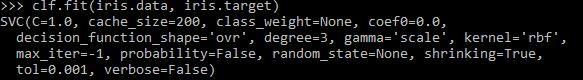
\includegraphics[width=0.75\textwidth]{figures/huda/21.JPG}}\caption{Hasil Tampilan 12.}\end{figure}
\begin{figure}[ht]\centerline{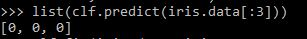
\includegraphics[width=0.75\textwidth]{figures/huda/22.JPG}}\caption{Hasil Tampilan 13.}\end{figure}
\begin{figure}[ht]\centerline{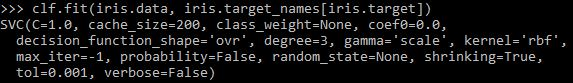
\includegraphics[width=0.75\textwidth]{figures/huda/23.JPG}}\caption{Hasil Tampilan 14.}\end{figure}
\begin{figure}[ht]\centerline{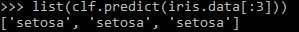
\includegraphics[width=0.75\textwidth]{figures/huda/24.JPG}}\caption{Hasil Tampilan 15.}\end{figure}
\begin{figure}[ht]\centerline{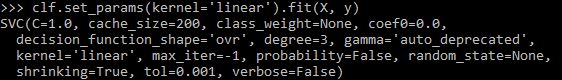
\includegraphics[width=0.75\textwidth]{figures/huda/25.JPG}}\caption{Hasil Tampilan 16.}\end{figure}
\begin{figure}[ht]\centerline{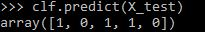
\includegraphics[width=0.75\textwidth]{figures/huda/26.JPG}}\caption{Hasil Tampilan 17.}\end{figure}
\begin{figure}[ht]\centerline{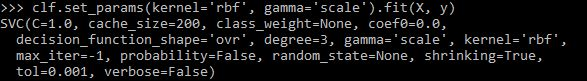
\includegraphics[width=0.75\textwidth]{figures/huda/27.JPG}}\caption{Hasil Tampilan 18.}\end{figure}
\begin{figure}[ht]\centerline{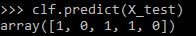
\includegraphics[width=0.75\textwidth]{figures/huda/28.JPG}}\caption{Hasil Tampilan 19.}\end{figure}
\begin{figure}[ht]\centerline{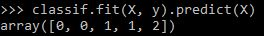
\includegraphics[width=0.75\textwidth]{figures/huda/29.JPG}}\caption{Hasil Tampilan 20.}\end{figure}
\begin{figure}[ht]\centerline{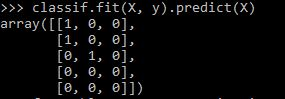
\includegraphics[width=0.75\textwidth]{figures/huda/30.JPG}}\caption{Hasil Tampilan 21.}\end{figure}
\begin{figure}[ht]\centerline{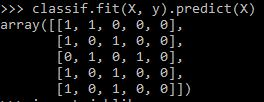
\includegraphics[width=0.75\textwidth]{figures/huda/31.JPG}}\caption{Hasil Tampilan 22.}\end{figure}

